\chapter{บทนำและหลักการฟิสิกส์เชิงแสง}
\label{chap:ch01}

\section*{แผนบริหารการสอนประจำบทที่ 1}
\addcontentsline{toc}{section}{แผนบริหารการสอนประจำบทที่ 1}

\begin{planbox}{หัวข้อเนื้อหาประจำบท}
\begin{enumerate}[leftmargin=1.5em, itemsep=1pt]
    \item ความสำคัญของการตรวจวัดธาตุอาหารดินในการเกษตรแม่นยำ
    \item หลักการทางทัศนศาสตร์ฟิสิกส์และกฎของเบียร์และแลมเบิร์ต
    \item การจำแนกแถบสเปกตรัมแสงสำหรับการตรวจวัดธาตุไนโตรเจน ฟอสฟอรัส และโพแทสเซียม
    \item ทฤษฎีการลดทอนแสงและความสัมพันธ์กับดัชนีหักเหและความหนาแน่นของของเหลว
\end{enumerate}
\end{planbox}

\begin{planbox}{วัตถุประสงค์เชิงพฤติกรรม}
\begin{enumerate}[leftmargin=1.5em, itemsep=1pt]
    \item อธิบายหลักการทางฟิสิกส์ของการดูดกลืนแสงตามกฎของเบียร์และแลมเบิร์ตได้อย่างถูกต้อง
    \item จำแนกความยาวคลื่นที่เหมาะสมในการทำปฏิกิริยากับสารละลายธาตุอาหารดินได้อย่างสมบูรณ์
    \item อธิบายความสัมพันธ์ระหว่างการลดทอนแสงกับดัชนีหักเหและความหนาแน่นของของเหลวได้อย่างถูกต้อง
\end{enumerate}
\end{planbox}

\begin{planbox}{กิจกรรมการเรียนการสอน}
\begin{enumerate}[leftmargin=1.5em, itemsep=1pt]
    \item การบรรยายเชิงทฤษฎีประกอบการฉายสื่อแอนิเมชันการแผ่และดูดกลืนคลื่นแม่เหล็กไฟฟ้า
    \item การสาธิตการทำงานของเครื่องสเปกโทรโฟโตมิเตอร์ตรวจวัดสารละลายตัวอย่างจริง
    \item การอภิปรายกลุ่มย่อยเกี่ยวกับการประยุกต์ทัศนศาสตร์ฟิสิกส์ในงานเกษตรดิจิทัล
\end{enumerate}
\end{planbox}

\begin{planbox}{สื่อการเรียนการสอน}
\begin{enumerate}[leftmargin=1.5em, itemsep=1pt]
    \item เอกสารคำสอนและสไลด์บรรยายบทที่ 1
    \item เครื่องสเปกโทรโฟโตมิเตอร์ NPK Level Meter 1.02 และหลอดคิวเวตต์มาตรฐาน
    \item ชุดสารละลายมาตรฐานสีสำหรับการทดสอบการดูดกลืนแสง
\end{enumerate}
\end{planbox}

\begin{planbox}{การวัดและประเมินผล}
\begin{enumerate}[leftmargin=1.5em, itemsep=1pt]
    \item การประเมินความสนใจและการมีส่วนร่วมในการอภิปรายในชั้นเรียน
    \item การทดสอบย่อยวัดความรู้ความเข้าใจเรื่องกฎของเบียร์และแลมเบิร์ต
    \item การตรวจความถูกต้องของการตอบคำถามทบทวนท้ายบทที่ 1
\end{enumerate}
\end{planbox}

\clearpage

\section{ความสำคัญของการตรวจวัดธาตุอาหารดินในการเกษตรแม่นยำ}
การตรวจวัดปริมาณธาตุอาหารหลักในดินอันประกอบด้วยไนโตรเจน ฟอสฟอรัส และโพแทสเซียม หรือ NPK มีความสำคัญอย่างยิ่งต่อการบริหารจัดการธาตุอาหารพืชในการเกษตรแม่นยำ (Precision Agriculture) โดยเฉพาะในพื้นที่ปลูกไม้ผลเศรษฐกิจ เช่น ทุเรียนแปลงใหญ่ การตรวจวัดในภาคสนามที่ต้องการความรวดเร็วและแม่นยำสูงสามารถดำเนินการได้ด้วยเทคนิคการดูดกลืนแสงเชิงสเปกตรัม (Optical Absorption Spectroscopy)

\begin{figure}[H]
    \centering
    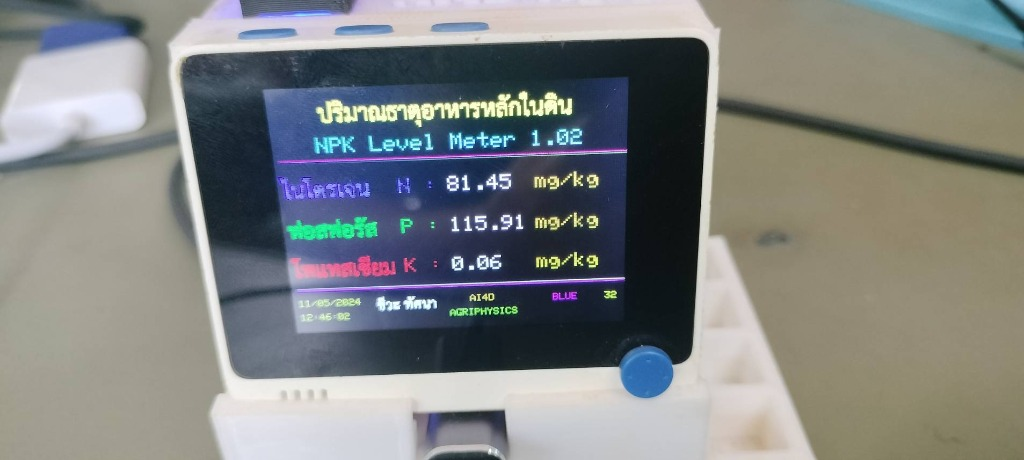
\includegraphics[width=0.70\textwidth]{images/device_overview.jpg}
    \caption{เครื่องสเปกโทรโฟโตมิเตอร์ตรวจวัดธาตุอาหารหลักในดิน NPK Level Meter 1.02}
    \label{fig:device_overview}
\end{figure}

\section{กฎของเบียร์และแลมเบิร์ต}
เมื่อลำแสงเอกรงค์ (Monochromatic Light) หรือแสงที่มีความยาวคลื่นจำเพาะส่องผ่านสารละลายตัวอย่างดินที่ผ่านกระบวนการทำปฏิกิริยาเกิดสี ความเข้มของแสงที่ทะลุผ่านจะลดลงตามความเข้มข้นของสารละลายและความหนาของชั้นสารละลายตามความสัมพันธ์

\begin{equation}
    A(\lambda) = -\log_{10}\left(\frac{I(\lambda) - I_{\text{dark}}}{I_0(\lambda) - I_{\text{dark}}}\right) = \varepsilon(\lambda) \cdot b \cdot C
\end{equation}

กำหนดให้
\begin{itemize}[leftmargin=2.0em, itemsep=2pt]
    \item $A(\lambda)$ แทนค่าการดูดกลืนแสง (Absorbance) ณ ความยาวคลื่น $\lambda$
    \item $I_0(\lambda)$ แทนความเข้มแสงเริ่มต้นที่ส่องผ่านสารละลายแบลงก์ (Blank Reference)
    \item $I(\lambda)$ แทนความเข้มแสงที่ทะลุผ่านสารละลายตัวอย่าง (Sample Transmitted Intensity)
    \item $I_{\text{dark}}$ แทนสัญญาณกระแสมืดของเซนเซอร์ขณะดับไฟ (Dark Current)
    \item $\varepsilon(\lambda)$ แทนสัมประสิทธิ์การดูดกลืนแสงโมลาร์ (Molar Absorptivity)
    \item $b$ แทนความยาวของทางเดินแสงในคิวเวตต์ มีค่าเท่ากับ 1.0 เซนติเมตร
    \item $C$ แทนความเข้มข้นของธาตุอาหารในสารละลาย มีหน่วยเป็นมิลลิกรัมต่อกิโลกรัม ($\text{mg/kg}$)
\end{itemize}

\section{การจำแนกความยาวคลื่นสำหรับการวัด NPK}
ระบบสเปกโทรโฟโตมิเตอร์เครื่องนี้ใช้แหล่งกำเนิดแสงแบบหลายความยาวคลื่นผ่านโมดูลไดโอดเปล่งแสงหลายสีดิจิทัล WS2812B ร่วมกับเซนเซอร์วัดค่าสีแบบดิจิทัล TCS34725 ซึ่งสามารถแยกแยะช่องสัญญาณแสงตามความยาวคลื่นหลักได้ดังนี้

\begin{enumerate}[leftmargin=1.5em, itemsep=3pt]
    \item \textbf{แสงสีน้ำเงิน (Blue Spectrum ความยาวคลื่น 465 นาโนเมตร)} ใช้สำหรับการตรวจวัดความเข้มข้นของธาตุไนโตรเจน (Nitrogen หรือ N) ซึ่งทำปฏิกิริยากับน้ำยาทดสอบเกิดสารประกอบสีส้มอมน้ำตาล
    \item \textbf{แสงสีฟ้าอมเขียว (Cyan Spectrum ความยาวคลื่น 500 นาโนเมตร)} ใช้สำหรับการวิเคราะห์สารประกอบอินทรีย์และการดูดกลืนแสงช่วงกลาง
    \item \textbf{แสงสีเขียว (Green Spectrum ความยาวคลื่น 525 นาโนเมตร)} ใช้สำหรับการตรวจวัดความเข้มข้นของธาตุฟอสฟอรัส (Phosphorus หรือ P) ซึ่งทำปฏิกิริยากับน้ำยาทดสอบเกิดสารประกอบเชิงซ้อนสีน้ำเงินโมลิบดีนัม
    \item \textbf{แสงสีเหลือง (Yellow Spectrum ความยาวคลื่น 590 นาโนเมตร)} ใช้สำหรับการตรวจวัดค่าความขุ่นและอนุภาคแขวนลอยในสารละลาย
    \item \textbf{แสงสีแดง (Red Spectrum ความยาวคลื่น 625 นาโนเมตร)} ใช้สำหรับการตรวจวัดความเข้มข้นของธาตุโพแทสเซียม (Potassium หรือ K) ซึ่งทำให้เกิดความขุ่นและการสะท้อนแสงของตะกอนเตตระฟีนิลบอเรต
    \item \textbf{แสงสีขาว (White Spectrum ความยาวคลื่นครอบคลุม 400 ถึง 700 นาโนเมตร)} ใช้สำหรับการเทียบมาตรฐานศูนย์ (Blank Calibration) และการตรวจวัดค่าความขุ่นรวมของสารละลายดิน
\end{enumerate}

\section{การวิเคราะห์สมบัติเชิงทัศนศาสตร์และมาตรวิทยาของเหลว}
นอกเหนือจากการตรวจวัดธาตุอาหารในดินแล้ว ระบบยังได้รับการพัฒนาขยายขีดความสามารถสู่การเป็นเครื่องตรวจวิเคราะห์สมบัติเชิงแสงและกายภาพของตัวอย่างของเหลวทางการเกษตร (Liquid Optics \& Metrology) เช่น น้ำชลประทาน น้ำหมักชีวภาพ และสารละลายธาตุอาหารพืช โดยอาศัยหลักการความสัมพันธ์ระหว่างการลดทอนแสง (Optical Attenuation) กับดัชนีหักเหของแสง (Refractive Index, $n$) และความหนาแน่นของของเหลว ($\rho$) ตามมาตรฐานสากล ICUMSA และทฤษฎี Lorentz-Lorenz \& Gladstone-Dale

\begin{equation}
    n = 1.3330 + 0.00143 \cdot (\text{Brix}) + 0.0000045 \cdot (\text{Brix})^2
\end{equation}

\begin{equation}
    \rho = 0.9982 + 0.00385 \cdot (\text{Brix}) + 0.000012 \cdot (\text{Brix})^2 \quad (\text{g/cm}^3)
\end{equation}

โดยที่น้ำกลั่นบริสุทธิ์มีค่าดัชนีหักเห $n = 1.3330$ และความหนาแน่น $\rho = 0.9982\text{ g/cm}^3$ ที่อุณหภูมิห้อง 20 องศาเซลเซียส

\section*{บทสรุปประจำบทที่ 1}
\addcontentsline{toc}{section}{บทสรุปประจำบทที่ 1}
การตรวจวัดธาตุอาหารหลักในดิน NPK และสมบัติของเหลวด้วยเทคนิคสเปกโทรโฟโตเมตรี อาศัยหลักการการลดทอนของความเข้มแสงเมื่อส่องผ่านตัวกลางตามกฎของเบียร์และแลมเบิร์ต แหล่งกำเนิดแสงดิจิทัล WS2812B ร่วมกับเซนเซอร์ TCS34725 ช่วยให้สามารถเลือกปล่อยแสงความยาวคลื่นจำเพาะ 465, 500, 525, 590 และ 625 นาโนเมตรได้อย่างแม่นยำ พร้อมทั้งสามารถประเมินสมบัติเชิงกายภาพของของเหลว ทั้งดัชนีหักเห ความหนาแน่น และระดับความเข้มข้นสารละลาย ได้อย่างมีประสิทธิภาพบนอุปกรณ์พกพาขนาดกะทัดรัด

\section*{คำถามทบทวนท้ายบทที่ 1}
\addcontentsline{toc}{section}{คำถามทบทวนท้ายบทที่ 1}
\begin{enumerate}[leftmargin=1.5em, itemsep=3pt]
    \item จงอธิบายหลักการทางฟิสิกส์ของกฎของเบียร์และแลมเบิร์ต และระบุข้อจำกัดในการนำกฎนี้ไปประยุกต์ใช้กับสารละลายตัวอย่างดินที่มีความขุ่นสูง
    \item เหตุใดการตรวจวัดธาตุไนโตรเจน (N) และฟอสฟอรัส (P) จึงต้องใช้ความยาวคลื่นแสงที่แตกต่างกัน จงอธิบายความสัมพันธ์กับสารประกอบเชิงซ้อนที่เกิดขึ้น
    \item สัญญาณกระแสมืด (Dark Current) คืออะไร และเหตุใดระบบเฟิร์มแวร์จึงต้องทำการดับไฟเพื่อวัดกระแสมืดก่อนทำการกวาดสเปกตรัมแสงทุกครั้ง
    \item จงอธิบายความสัมพันธ์ระหว่างค่าการดูดกลืนแสงเฉลี่ย ($A_{\text{mean}}$) ดัชนีหักเห ($n$) และความหนาแน่น ($\rho$) ของของเหลวตามมาตรฐาน ICUMSA
\end{enumerate}
